\documentclass{beamer}

\usetheme[sectionpage=simple, subsectionpage=simple,
numbering=fraction, progressbar=none]
{metropolis}

\usepackage[utf8]{inputenc}
\usepackage{graphicx}
\graphicspath{{./img/}}
\usepackage{tikz}

\title{Distributions of sampling statistics}
\date{\today}
\author{Gonzalo G. Peraza Mues}
% \institute{Universidad Politécnica de Yucatán}

\titlegraphic{
\includegraphics[height=1.5cm]{logo-upy}}

\newcommand{\E}[1]{\operatorname{E}\left[#1\right]}
\newcommand{\Var}[1]{\operatorname{Var}\left(#1\right)}
\renewcommand{\P}[1]{P\left(#1\right)}


\begin{document}
\maketitle
\begin{frame}{Sampling from a population}
  The measurable values of the items in the population can be thought of as
  being independent random variables from the underlying population
  distribution.

  If $X_1,\ldots,X_n$ are independent random variables having a common
  distribution $F$, they constitute a \alert{sample} from the distribution $F$.
\end{frame}

\begin{frame}{Inference}
  \textbf{Objective:} We want to learn about the population distribution by
  observing the sampled data.

  \alert{Parametric inference}: The form of the underlying distribution
  is specified up to a set of unknown parameters.

  \alert{Non-parametric inference}: Nothing is assumed about the form of F.
\end{frame}

\begin{frame}{Distribution of statistics}
  \alert{Statistic}: A random variable whose value is determined by the sample
  data. For example: the sample mean and the sample variance.
\end{frame}

\begin{frame}{The sample mean}
  Let $X_1,X_2,\ldots,X_n$ be a sample of values from a population with
  \alert{population mean} $\mu$ and \alert{population variance} $\sigma^2$. The
  sample mean is defined by
  \begin{align*}
    \bar{X} = \frac{X_1+\cdots+X_n}{n}
  \end{align*}

  $\bar{X}$ is a random variable with:
  \begin{align*}
    \E{\bar{X}} =& \E{\frac{X_1+\cdots+X_n}{n}} = \frac{n\mu}{n} = \mu\\
    \Var{\bar{X}} = & \Var{\frac{X_1+\cdots+X_n}{n}} = \frac{n\sigma^2}{n^2}
                      = \frac{\sigma^2}{n}
  \end{align*}
\end{frame}

\begin{frame}{The standard error}
  The standard error of a statistic is its standard deviation.

  The standard error of the mean (\alert{SEM}) is
  \begin{align*}
    SEM = SD(\bar{X}) = \frac{\sigma}{\sqrt{n}}
  \end{align*}

  $\bar{X}$ is centered about the population mean $\mu$, but its spread becomes
  more and more reduced as the sample size increases.

  The SEM can be approximated by $s/\sqrt{n}$.
\end{frame}

\begin{frame}{Density of sample means from a standard normal population}
  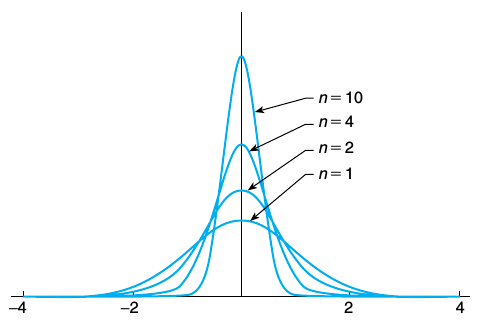
\includegraphics[width=\linewidth]{dpf-sample-mean}
\end{frame}

\begin{frame}{The Central Limit Theorem}
  Let $X_1,X_2,\ldots,X_n$ be a sequence of independent and identically
  distributed random variables each having mean $\mu$ and variance
  $\sigma^2$. Then for $n$ large, the distribution of
  \begin{align*}
    X_1 + \cdots + X_n
  \end{align*}
  is approximately normal with mean $n\mu$ and variance $n\sigma^2$.

  For $n$ large
  \begin{align*}
    \P{\frac{X_1+\cdots+X_n - n\mu}{\sigma\sqrt{n}}<x} \approx \P{Z<x}
  \end{align*}

  \begin{center}
    \href{http://students.brown.edu/seeing-theory/distributions/index.html\#third}{Web
      simulation}
  \end{center}
\end{frame}

\begin{frame}[t,shrink=10]{Example R6.3a}
  An insurance company has 25,000 automobile policy holders. If the yearly
  claim of a policy holder is a random variable with mean 320 and standard
  deviation 540, approximate the probability that the total yearly claim exceeds
  8.3 million.
\end{frame}

\begin{frame}[t,shrink=15]{Example R6.3b. Homework}
  Civil engineers believe that $W$, the amount of weight (in units of 1,000
  pounds) that a certain span of a bridge can withstand without structural
  damage resulting, is normally distributed with mean 400 and standard deviation
  40. Suppose that the weight (again, in units of 1,000 pounds) of a car is a
  random variable with mean 3 and standard deviation 0.3. How many cars would
  have to be on the bridge span for the probability of structural damage to
  exceed 0.1?
\end{frame}

\begin{frame}{Normal approximation of the binomial distribution}
  A $Bin(n,p)$ distribution can be seen as a sum of random variables
  $X=X_1+\cdots+X_n$ with $\E{X_i} = p$ and $\Var{X_i} = p(1-p)$. From the
  central limit theorem, for $n$ large
  \begin{align*}
    \frac{X-np}{\sqrt{np(1-p)}}
  \end{align*}
  will be approximately a standard normal random variable.

  The normal approximation will be good for $np(1-p)\geq 10$.
\end{frame}

\begin{frame}[t,shrink=10]{Example R6.3c}
  The ideal size of a first-year class at a particular college is 150 students.
  The college, knowing from past experience that, on the average, only 30
  percent of those accepted for admission will actually attend, uses a policy of
  approving the applications of 450 students. Compute the probability that more
  than 150 first-year students attend this college.
\end{frame}

\begin{frame}{Approximate Distribution of the Sample Mean}
  The sample mean
  \begin{align*}
    \bar{X}=\frac{\sum_{i=1}^n X_i}{n}
  \end{align*}
  is approximately normal for $n$ large.
  \begin{align*}
    \frac{\bar{X}-\mu}{\sigma/\sqrt{n}}
  \end{align*}
  has approximately a standard normal distribution.

  A general rule of thumb is that one can be confident of the normal
  approximation whenever $n\geq 30$.
\end{frame}

\begin{frame}[t,shrink=10]{Example R6.3d. Homework}
  The weights of a population of workers have mean 167 and standard deviation
  27.

  (a) If a sample of 36 workers is chosen, approximate the probability that the
  sample mean of their weights lies between 163 and 170.

  (b) Repeat part (a) when the sample is of size 144.
\end{frame}

\begin{frame}[t,shrink=10]{Example R6.3e}
  An astronomer wants to measure the distance from her observatory to a distant
  star. However, due to atmospheric disturbances, any measurement will not yield
  the exact distance $d$. As a result, the astronomer has decided to make a
  series of measurements and then use their average value as an estimate of the
  actual distance. If the astronomer believes that the values of the successive
  measurements are independent random variables with a mean of $d$ light years
  and a standard deviation of 2 light years, how many measurements need she make
  to be at least 95 percent certain that her estimate is accurate to within
  $\pm 0.5$ light years?
\end{frame}

\begin{frame}{The Sample Variance}
  \begin{align*}
    S^2 = \frac{\sum_{i=1}^n\left(X_i - \bar{X}\right)^2}{n-1}
  \end{align*}
  Remember that
  $\sum_{i=1}^n\left(x_i - \bar{x}\right)^2 = \sum_{i=1}^n x_i^2 - n\bar{x}^2$,
  then it can be proved that
  \begin{align*}
    \E{S^2} = \sigma^2
  \end{align*}

  The reason for the factor $n-1$ is to set the expected value of $S^2$ to be
  the population variance $\sigma^2$.
\end{frame}

\begin{frame}{Sampling Distributions from a Normal Population}
  If $X_1,\ldots,X_n$ is a sample from a normal population having mean $\mu$ and
  variance $\sigma^2$, then $\bar{X}$ and $S^2$ are independent random
  variables, with (Proof as homework.):
\begin{itemize}
\item $\bar{X}$ being normal with mean $\mu$ and variance $\sigma^2/n$
\item $(n-1)S^2/\sigma^2$ being chi-squared with $n-1$ degrees of freedom.
\end{itemize}


  The independence of $\bar{X}$ and $S^2$ is a unique property of the normal
  distributions.

  It can also be proved that
  \begin{align*}
    \sqrt{n}\frac{\bar{X}-\mu}{S}\propto t_{n-1}
  \end{align*}
\end{frame}

\begin{frame}[t,shrink=10]{Example R6.5a}
  The time it takes a central processing unit to process a certain type of job
  is normally distributed with mean 20 seconds and standard deviation 3
  seconds. If a sample of 15 such jobs is observed, what is the probability that
  the sample variance will exceed 12?
\end{frame}
\begin{frame}{Sampling from a Finite Population}
  Consider a population of $N$ elements and take $p$ to be the proportion of the
  population with a certain characteristic of interest. For a random sample of
  size $n$ let
  \begin{align*}
    X_i =
    \begin{cases}
      1&\text{if the ith member of the sample has the characteristic}\\
      0&\text{otherwise}
    \end{cases}
  \end{align*}
  and let $X=X_1+X_2+\cdots+X_n$. $X$ is a hypergeometric random variable
  $Hyper(N,Np,n)$.
\end{frame}

\begin{frame}{Sampling from a Finite Population}
  For $n$ large, we can approximate $X$ by a $Bin(n,p)$ distribution with
  $\E{X}=np$ and $SD(X)=\sqrt{np(1-p)}$.

  The, $\bar{X}=X/n$ is the proportion of the sample that has the characteristic
  and has
  \begin{align*}
    \E{\bar{X}} =& p\\
    SD(\bar{X}) =& \sqrt{p(1-p)/n}
  \end{align*}
\end{frame}

\begin{frame}[t,shrink=10]{Example 6.6a}
  Suppose that 45 percent of the population favors a certain candidate in an
  upcoming election. If a random sample of size 200 is chosen, find

  (a) the expected value and standard deviation of the number of members of the
  sample that favor the candidate;

  (b) the probability that more than half the members of the sample favor the
  candidate.
\end{frame}

\begin{frame}[t,shrink=10]{Example 6.6b}
  According to the U.S. Department of Agriculture’s ``World Livestock
  Situation'', the country with the greatest per capita consumption of pork is
  Denmark. In 1994, the amount of pork consumed by a person residing in Denmark
  had a mean value of 147 pounds with a standard deviation of 62 pounds. If a
  random sample of 25 Danes is chosen, approximate the probability that the
  average amount of pork consumed by the members of this group in 1994 exceeded
  150 pounds.

\end{frame}
\end{document}

%%% Local Variables:
%%% mode: latex
%%% TeX-master: t
%%% End:
